\chapter{Comparison of ML and Cut and Count (This is the shit, should find better title)}
\label{sec:results}
Until this point we have looked at how well the different analyses perform on the same dataset and we are now going to see how sensitive they are to the signal samples we have chosen. To be able to do this we have to know how we can quantify the sensitivity before we move on to our results. 
%\input{Sections/Results/CutAndCount/SlepSlep}
%%\section{Cut and count}
%\label{sec:resultsCandC}

\input{Sections/Results/CutAndCount/SlepSlep}




\input{Sections/Results/CutAndCount/C1C1_WW}

\input{Sections/Results/CutAndCount/Mono-Z}

%\section{Machine learning}
\label{sec:resultsML}

\subsection{BDT}
\label{sec:resultsBDT}

\subsubsection{MC simulated data}

\subsubsection{Real data}




\subsection{Neural networks}
\label{sec:resultsNN}

\subsubsection{MC simulated data}

\subsubsection{Real data}

\section{Quantifying the sensitivity}
\label{sec:significance}

The overall goal with the analysis carried out in this thesis is to optimize the sensitivity to discover new physics and possibly in the end to claim discovery of new particles. To check if we have succeeded in making our model sensitive to new physics we can check the expected p-values and significances for our signal region. 

Each event in the data will either pass or fail the cuts defining the signal region used in the analysis. The number of events therefore follows a binomial distribution, and the probability of finding $n$ events in our region is given by equation \ref{eq:pval1}. 

\begin{equation}
    \label{eq:pval1}
    P(n|N, p) = \frac{N!}{n!(N-n)!} p^n(1-p)^{N-n},
\end{equation}

where $N$ is the number of total events and p is the probability for the event to pass the cuts. If the number of total events gets very big and the probability $p$ gets very small, we can approximate equation \ref{eq:pval1} as a Poisson distribution, which is given by

\begin{equation}
    \label{eq:pval2}
    P(n|\nu) = \frac{\nu^n}{n!} e^{-\nu},
\end{equation}

where $\nu$ is given by a hypothesis. This equation (eq. \ref{eq:pval2}) gives us a probability of $n$ observed events when the expectation is to observe $\nu$ events. 

When we are talking about hypotheses in this thesis, we are talking about \textit{background-only} (b-only) and \textit{signal + background} (s+b) hypotheses. The b-only hypothesis is the SM, which is a well known theory. We are going to check this against the s+b hypothesis which in our case will be one of the three SUSY processes or the mono-Z process. This gives us the opportunity to introduce the p-values. A p-value is a measure to judge the deviation of the observed number of events from the b-only hypothesis expectations. If we assume that only the SM processes contribute we can use the p-value to get the probability of observing as many, or more, events as we can find in the data. With a perfectly known background the p-value can be found by

\begin{equation}
    \label{eq:pvalues}
    p = \sum_{n=n_{obs}}^\infty f(n;b),
\end{equation}


where $f(n;b)$ is the Poisson distribution given in equation \ref{eq:pval2}. It is common to convert the p-value into an observed significance $z$ with a unit Gaussian $\Phi$. This is given by

\begin{equation}
    \label{eq:signifobs}
    z = \Phi^{-1}(1-p)
\end{equation}

 and the unit is expressed with a $\sigma$ as in number of standard deviations from the center of the Gaussian distribution. To claim discovery of a new particle we need an observed significance above 5 $\sigma$. We are not going to check the observed significance in this thesis, but calculate the expected significance to see if there is any hope to discover new physics for the models we are looking at. The expected significance is the significance associated with the median number of expected events under the s+b hypothesis. It gives us a number on how well the two hypotheses we are looking at are separated. This is given by equation \ref{eq:signif}, where the p-value now is expressed as a \textit{confidence level} (CL) given as
 
 \begin{equation}
    \label{eq:CL}
    CL_{s+b} = \sum_{n=0}^{q_{obs}} \frac{(s+b)^n}{n!} e^{-(s+b)},
 \end{equation}

where $q_{obs}$ is the number of observed events. If the $CL_{s+b}$ is below 5\% we exclude that we can find any new physics with the selection criteria we have given it. Putting equation \ref{eq:signifobs} and \ref{eq:CL} together we get the expression

\begin{equation}
    \label{eq:signif}
    Z_N = \Phi^{-1}(1-CL_{s+b}),
\end{equation}

where $Z_N$ is the expected significance. To claim exclusion in the signal region we need a $CL_{s+b} \leq$ 5\% which corresponds to $Z_N \leq 1.64 \sigma$. In this thesis the $Z_N$ is calculated by an already existing tool in ROOT called \texttt{RooStats.NumberCountingUtils.BinomialExpZ} which simply takes the number of events for both background and signal as input together with a fractional background uncertainty of e.g. 20\%.







\begin{comment}

\begin{equation}
    \label{eq:pval3}
    p = P(n \geq q_{obs}|b) \sum_{n=q_{obs}}^\infty \frac{b^n}{n!} e^{-b}
\end{equation}

As mentioned several times in this project the goal is to claim discovery of the Higgs boson. To do that we have to reject the b-only hypothesis. To do this we are going to use p-values and confidence levels. \\


which is a probability of finding $n$ events in our signal region. 









\textbf{P-values}\\
Assuming a null hypothesis to be true we can use the p-value as a function that quantifies how often we would obtain data as far away from the null hypothesis as the observed data. Since it is a function of the data, the p-value is of course a random variable. We have the p-values $p_0$ and $p_1$ for the hypotheses $H_0$ and $H_1$ which is given by 

\begin{equation}
    \label{eq:p0}
    p_0 = \int_{t_{obs}}^{+ \infty} g(t|H_0) dt,
\end{equation}
and
\begin{equation}
    \label{eq:p1}
    p_1 = \int_{t_{obs}}^{+ \infty} g(t|H_1) dt.
\end{equation}

These are probabilities to find the test statistic ($t$) values that are equal or greater than the observed test statistic ($t_{obs}$). The p-values can also be expressed by confidence levels as

\begin{equation}
    \label{eq:p0CL}
    p_0 = 1-CL_b
\end{equation}
and 
\begin{equation}
    \label{eq:p1CL}
    p_1 = CL_{s+b}.
\end{equation}

How to calculate the $CL_b$ and $CL_{s+b}$ is shown in equation \ref{eq:CLb} and \ref{eq:CLsb} later in this section.\\

\textbf{Confidence levels}\\
The method we are using to check if this is a good fit is confidence levels. The confidence level tells us how often the results will fit the expectations. E.g. a confidence level of 90\% tells us that the results fit the expectations 90\% of the time. In figure \ref{fig:CL} we can see an illustrative plot of the test statistic distribution with the confidence levels marked. 


\begin{figure}[H]
    \centering
    \includegraphics[width = 0.7\textwidth]{Figures/CL.png}
    \caption{This is a illustration of the test statistic distribution for the b-only and s+b hypotheses with the $CL_b$ and $CL_{s+b}$ marked. \cite{datanal}}
    \label{fig:CL}
\end{figure}

The compability of the observed test statistic, $t_{obs}$, with the two hypothesis, b-only and s+b, are defined as

\begin{equation}
    \label{eq:CLb}
    1 - CL_b = \int_{-\infty}^{t_{obs}} \text{g(t; b-only) dt}
\end{equation}

and

\begin{equation}
    \label{eq:CLsb}
    CL_{s+b} = \int_{t_{obs}}^{+\infty} \text{g(t; s+b) dt}.
\end{equation}



\textbf{Results for the p-values and confidence levels}\\
By using equation \ref{eq:CLb} and \ref{eq:CLsb} we get the following results



In table \ref{tab:CLZ} we can see the results for the p-values ($1-CL_b$) and the confidence levels. As we can see is the expected significance is below 5$\sigma$ so we did not expect to claim a discovery which also is compatible with the observed significance from the data. \\

We can also see that the value for $CL_{s+b}$ for the b-only hypothesis is below 0.05 which is the limit for excluding this hypothesis but since the observed value is $> 0.05$ we can't exclude it either.  



\begin{table}[H]
    \centering
    \begin{tabular}{c c c}\hline
     & 1-CL_b & CL_{s+b}\\\hline\hline
    b-only     &  & \\
    s+b     &  &\\
    data &  & \\\hline
    \end{tabular}
    \caption{Caption}
    \label{tab:CL}
\end{table}


\begin{table}[H]
    \centering
    \begin{tabular}{c c}\hline
     & CL$_{s+b}$ \\\hline\hline
    Median s+b experiment     &  0.500\\
    Median b-only experiment     & 0.023\\
    Data & 0.843\\\hline
    \end{tabular}
    \caption{Caption}
    \label{tab:my_label}
\end{table}


\end{comment}



\section{Results}
In this section the results of the expected significance for all four processes and the three analysis methods are presented. They are calculated as described in the previous section, but for the ML methods we have done one more step. We have found where we can get most sensitivity for the three benchmark signals for each process by looking at each bin in figure \ref{fig:BDTdataAll} and \ref{fig:NNdataAll}. This is done by calculating the significance for all bins, then cut away the first bin, then the second bin and so on. Then we see which bin we got the best significance at, and use this bin to calculate the significance for all signals in the respective mass splitting. Which bin that is used for each optimization varies a bit, but is usually within the last 1/10 of the bins in figure \ref{fig:BDTdataAll} and \ref{fig:NNdataAll}. This we can also expect since we can see that we have a lot more signal in this region of the output than in the first bins. 

\subsection{Direct slepton production}
\label{sec:resSlepSlep}
The first results we are going to look at is for the direct slepton production. The results are presented in figure \ref{fig:signAllSlepSlep}, where we have the mass of the slepton on the x-axis and the mass of the neutralino on the y-axis. 

\begin{figure}[H]
    \centering
    \begin{subfigure}[t!]{0.49\textwidth}
    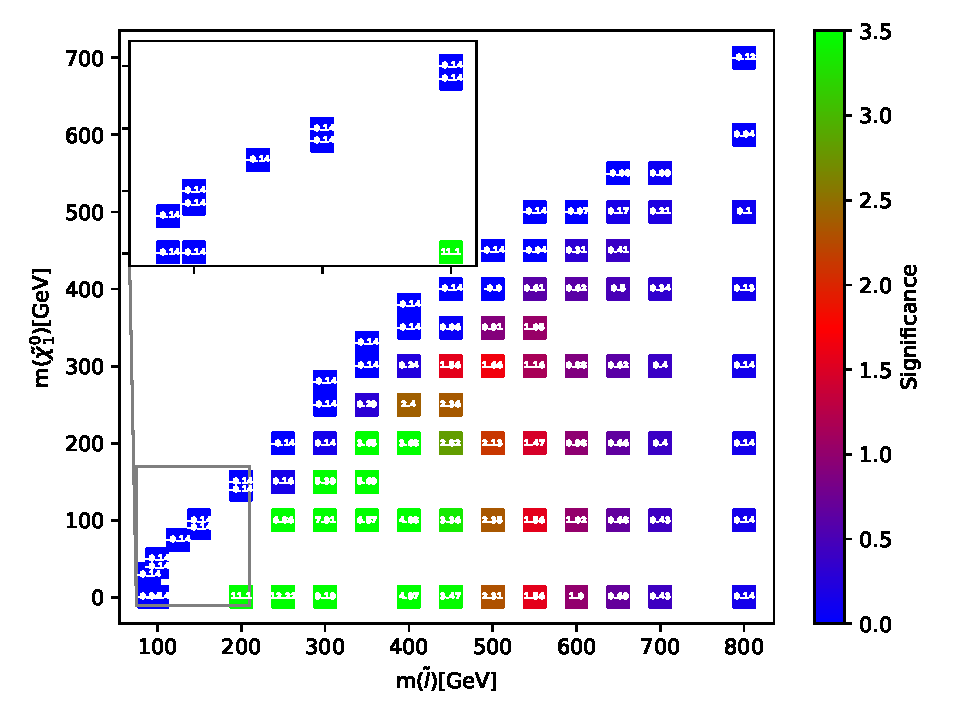
\includegraphics[width = \textwidth]{Figures/Significances/significanceCutandCount_slepslep_all.pdf}
    \caption{Cut and count.}
        \label{fig:signAllSlepSlepcandc}
    \end{subfigure}
    \\
    \begin{subfigure}[t!]{0.49\textwidth}
    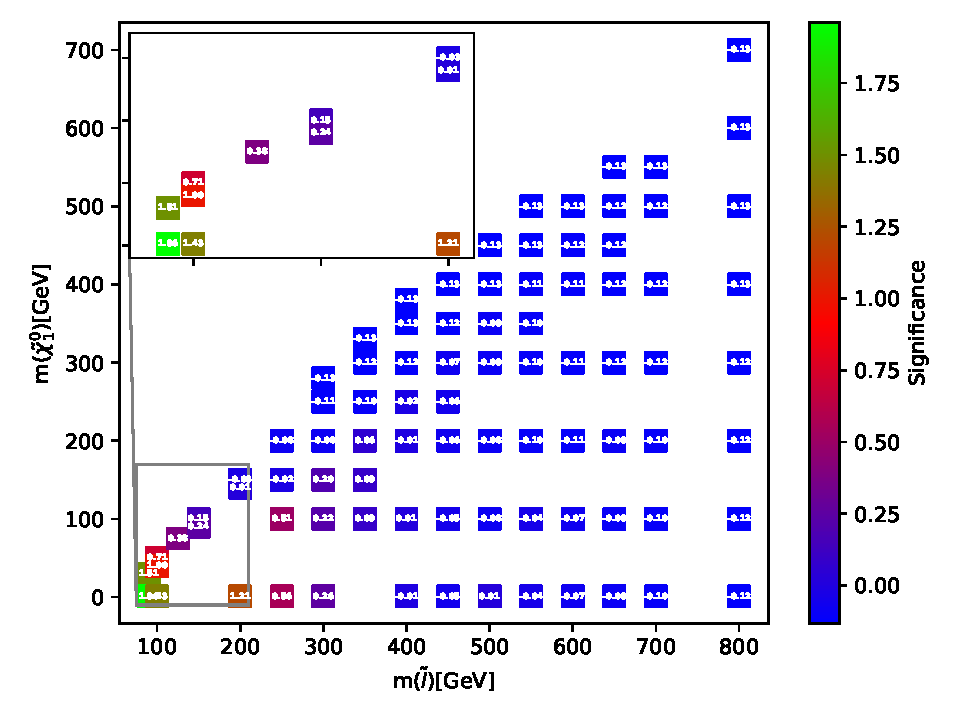
\includegraphics[width = \textwidth]{Figures/Significances/significance_BDT_slepslep_All_level.pdf}
    \caption{Boosted Decision Tree.}
        \label{fig:signAllSlepSlepBDT}
    \end{subfigure}      
    \begin{subfigure}[t!]{0.49\textwidth}
    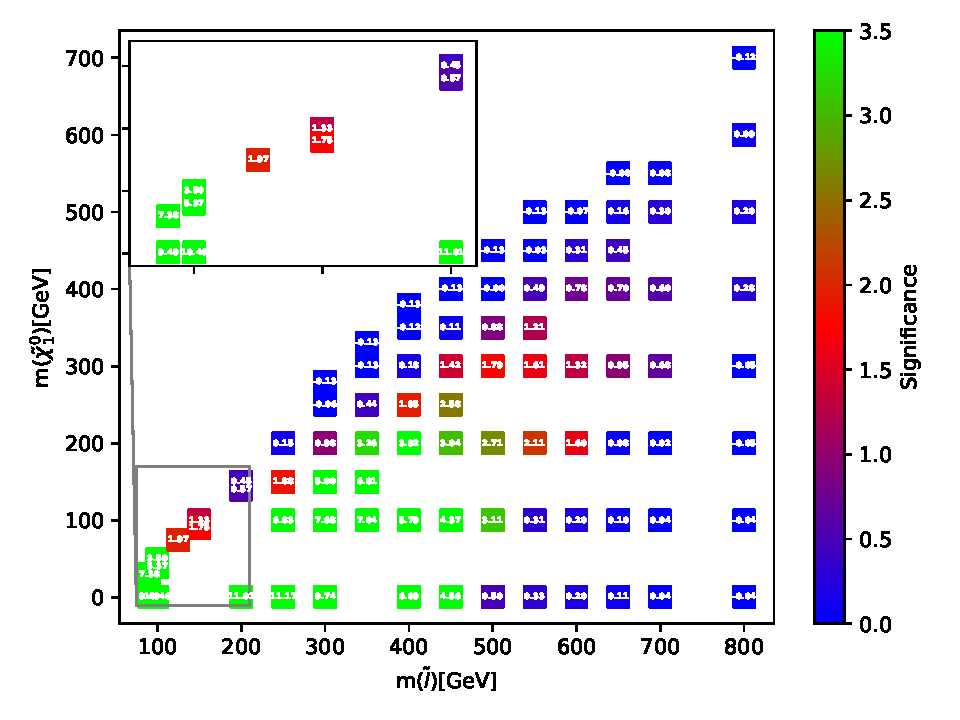
\includegraphics[width = \textwidth]{Figures/Significances/significance_NN_slepslep_All_level.pdf}
    \caption{Neural Network.}
        \label{fig:signAllSlepSlepNN}
    \end{subfigure}
    \caption{Significance plots for direct slepton production where all features are used during training the ML models.}
    \label{fig:signAllSlepSlep}
\end{figure}

This figure shows the expected significance for cut and count (\ref{fig:signAllSlepSlepcandc}), BDT (\ref{fig:signAllSlepSlepBDT}) and NN (\ref{fig:signAllSlepSlepNN}). The color bar is fixed in all plots to make it easier to compare the different results. As we can see, the expected significance is greater for several signal samples for both the BDT and NN than for the cut and count method. In particular, signal samples with low mass splittings ($\Delta m \leq 100$ GeV) show big improvements for both ML methods compared to cut and count. As stated in section \ref{sec:summary_ML} signals with low mass splittings are particularly hard to distinguish from SM background, making these results very interesting.












\subsection{Chargino pair with slepton/sneutrino-mediated-decay}
\label{sec:resC1C1_SlepSnu}

The results for the chargino production with slepton/sneutrino-mediated-decay are presented in figure \ref{fig:signAllslepsnu}. Here are the x-axis the mass of the chargino, while the y-axis remains the mass of the neutralino.

\begin{figure}[H]
    \centering
    \begin{subfigure}[t!]{0.49\textwidth}
    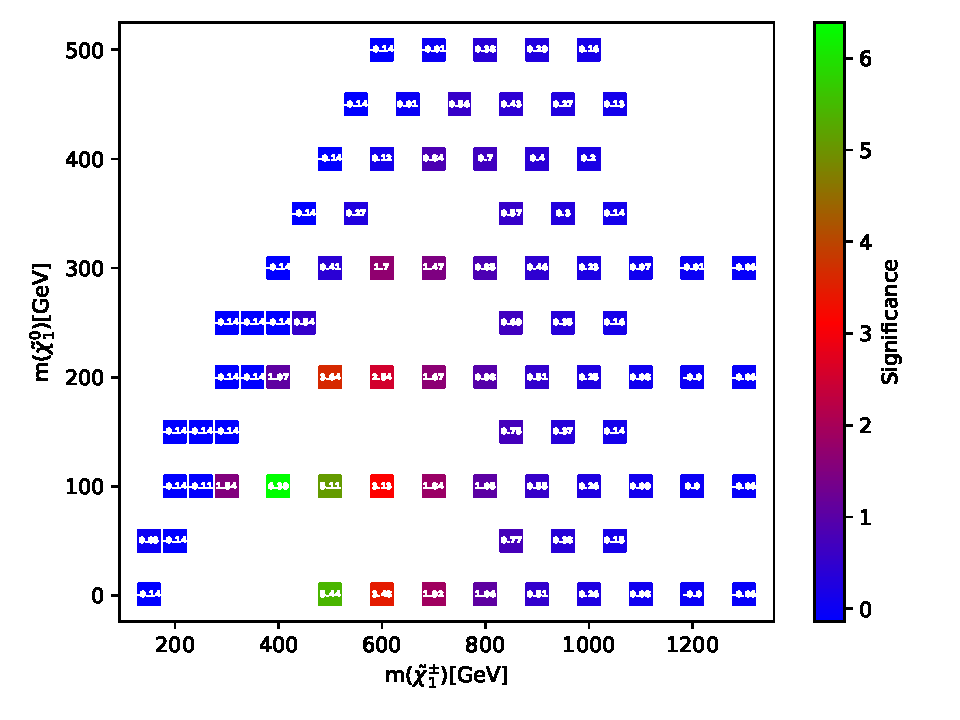
\includegraphics[width = \textwidth]{Figures/Significances/significanceCutandCount_slepsnu_all.pdf}
    \caption{Cut and count.}
        \label{fig:signAllslepsnucandc}
    \end{subfigure}
    \\
    \begin{subfigure}[t!]{0.49\textwidth}
    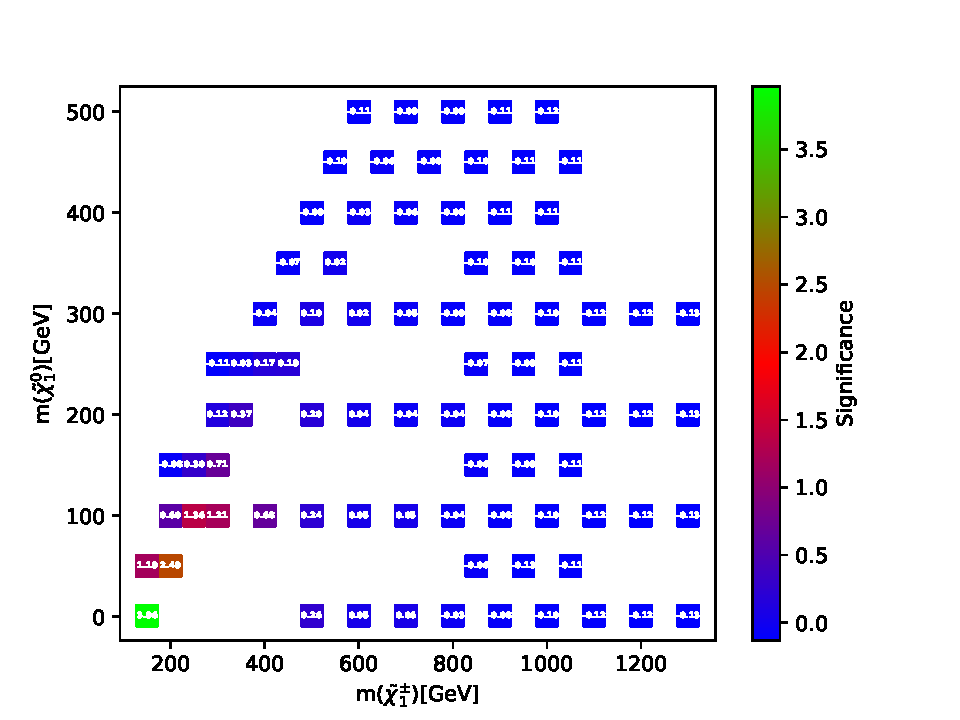
\includegraphics[width = \textwidth]{Figures/Significances/significance_BDT_slepsnu_All_level.pdf}
    \caption{Boosted Decision Tree.}
        \label{fig:signAllslepsnuBDT}
    \end{subfigure}      
    \begin{subfigure}[t!]{0.49\textwidth}
    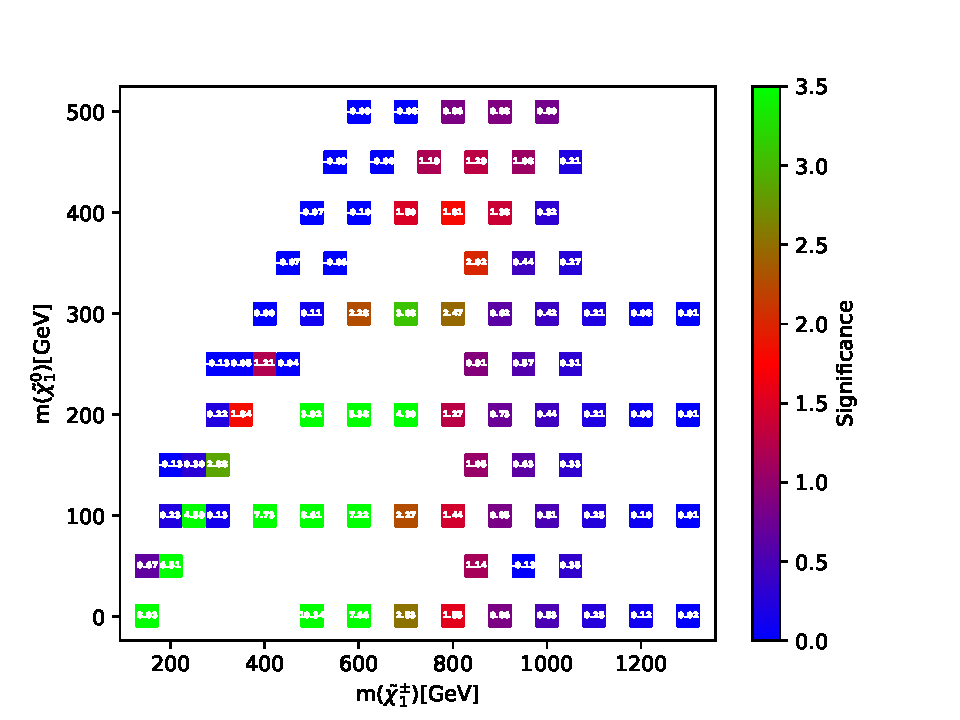
\includegraphics[width = \textwidth]{Figures/Significances/significance_NN_slepsnu_All_level.pdf}
    \caption{Neural Network.}
        \label{fig:signAllslepsnuNN}
    \end{subfigure}
    \caption{Significance plots for chargino production with slepton/sneutrino-mediated-decay where all features are used during training the ML models.}
    \label{fig:signAllslepsnu}
\end{figure}

Figure \ref{fig:signAllslepsnu} shows the expected significance for all three analysis methods used in this thesis. As for the direct slepton production, we can see that the ML have a greater sensitivity than the cut and count. The ML methods also have a greater sensitivity for low mass splittings ($\Delta m < 200$ GeV) compared to cut and count. 





























\subsection{Chargino pair with W-boson-mediated-decay}
\label{sec:resC1C1_WW}

The next results we are going to look at are for the chargino production with W-boson-mediated-decay, which are presented in figure \ref{fig:signAllWW}. The x- and y-axis are the same as for the chargino production with slepton/sneutrino-mediated-decay. 

\begin{figure}[H]
    \centering
    \begin{subfigure}[t!]{0.49\textwidth}
    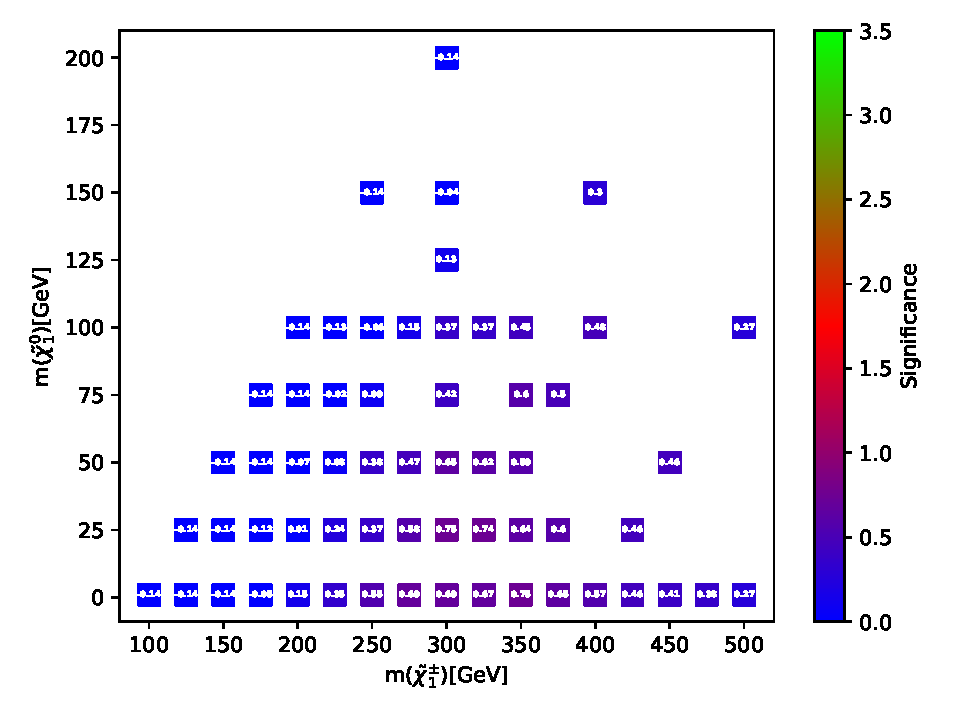
\includegraphics[width = \textwidth]{Figures/Significances/significanceCutandCount_WW_all.pdf}
    \caption{Cut and count.}
        \label{fig:signAllWWcandc}
    \end{subfigure}
    \\
    \begin{subfigure}[t!]{0.49\textwidth}
    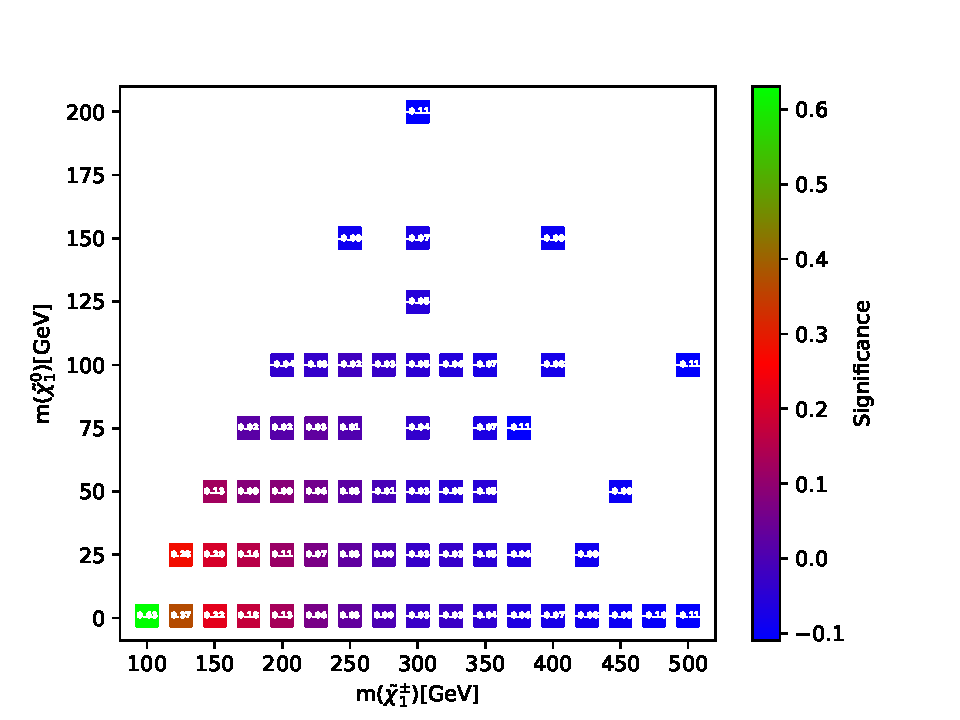
\includegraphics[width = \textwidth]{Figures/Significances/significance_BDT_WW_All_level.pdf}
    \caption{Boosted Decision Tree.}
        \label{fig:signAllWWBDT}
    \end{subfigure}      
    \begin{subfigure}[t!]{0.49\textwidth}
    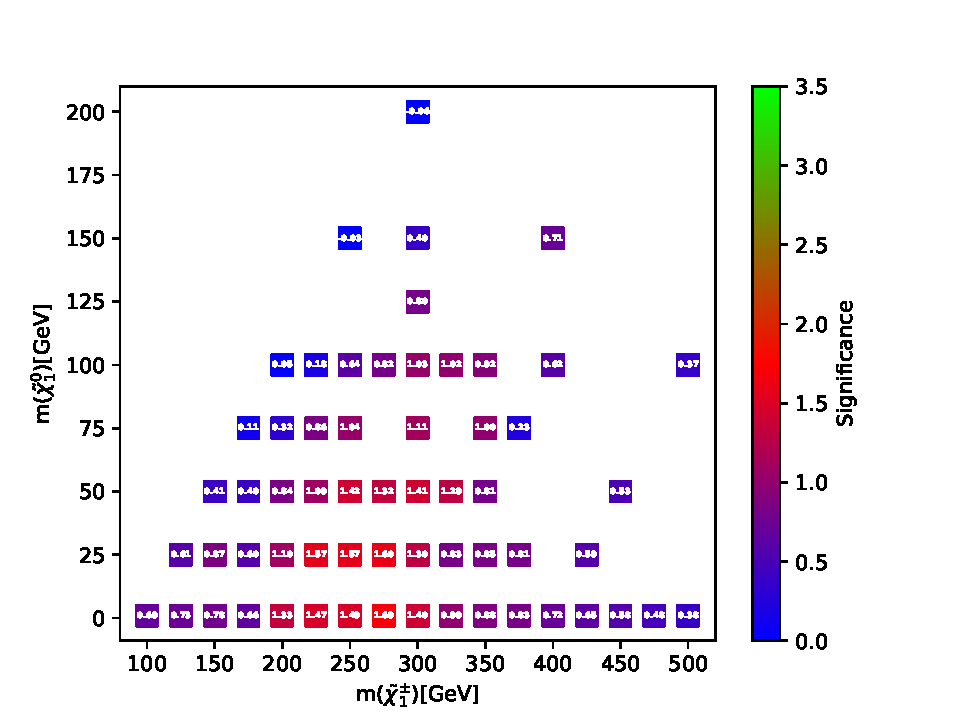
\includegraphics[width = \textwidth]{Figures/Significances/significance_NN_WW_All_level.pdf}
    \caption{Neural Network.}
        \label{fig:signAllWWNN}
    \end{subfigure}
    \caption{Significance plots for chargino production with W-boson-mediated-decay where all features are used during training the ML models.}
    \label{fig:signAllWW}
\end{figure}

From figure \ref{fig:signAllWW}, we can easily see that the sensitivity are better for most signal samples for the ML methods than the cut and count method. However, the sensitivity all over is not that good, and we should not expect to do any discovery at any mass splitting. 


































\subsection{Mono-Z}
\label{sec:resMono-Z}

The last results we are going to look at is for the mono-Z process. The results are presented in figure \ref{fig:signAllmonoZ}, where we have the mass of the mediator on the x-axis and the mass of the DM particle on the y-axis. 

\begin{figure}[H]
    \centering
    \begin{subfigure}[t!]{0.49\textwidth}
    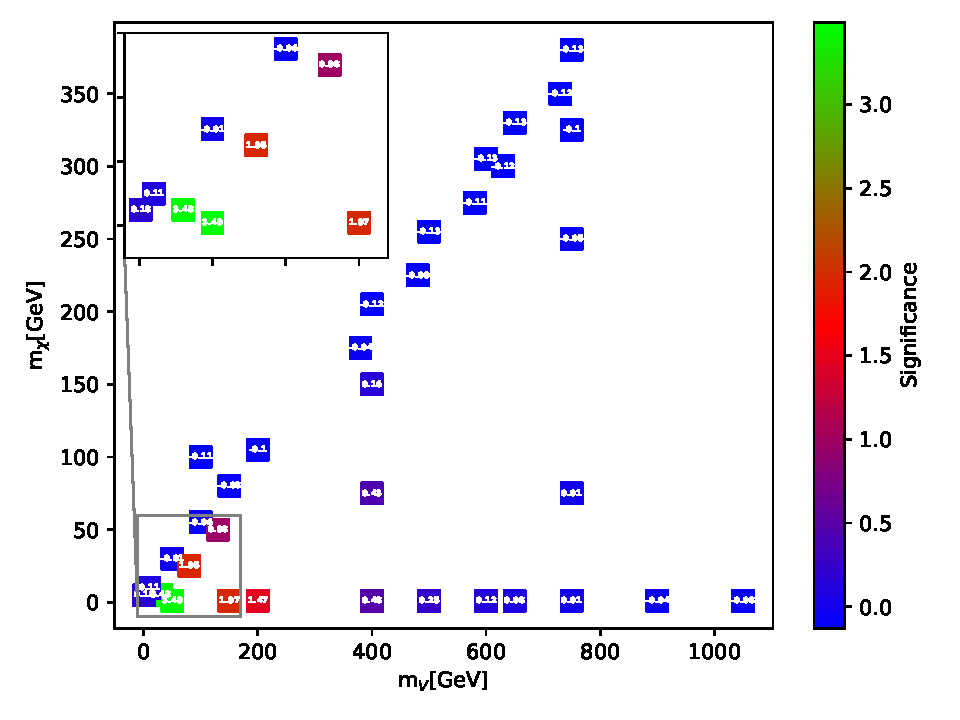
\includegraphics[width = \textwidth]{Figures/Significances/significanceCutandCount_monoZ_all.pdf}
    \caption{Cut and count.}
        \label{fig:signAllmonoZcandc}
    \end{subfigure}
    \\
    \begin{subfigure}[t!]{0.49\textwidth}
    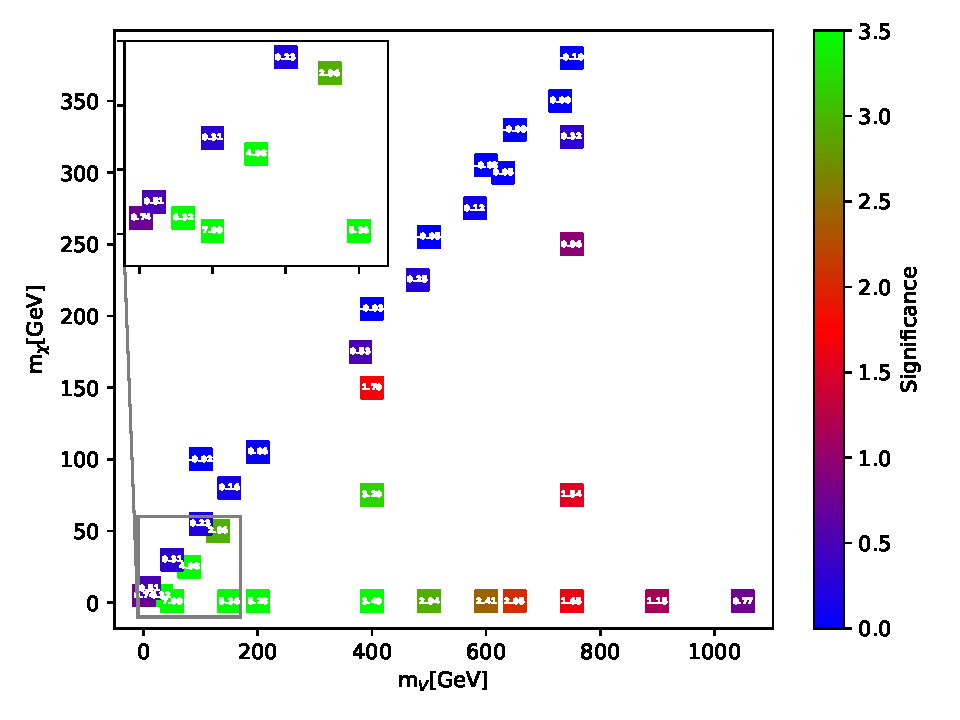
\includegraphics[width = \textwidth]{Figures/Significances/significance_BDT_monoZ_All_level.pdf}
    \caption{Boosted Decision Tree.}
        \label{fig:signAllmonoZBDT}
    \end{subfigure}      
    \begin{subfigure}[t!]{0.49\textwidth}
    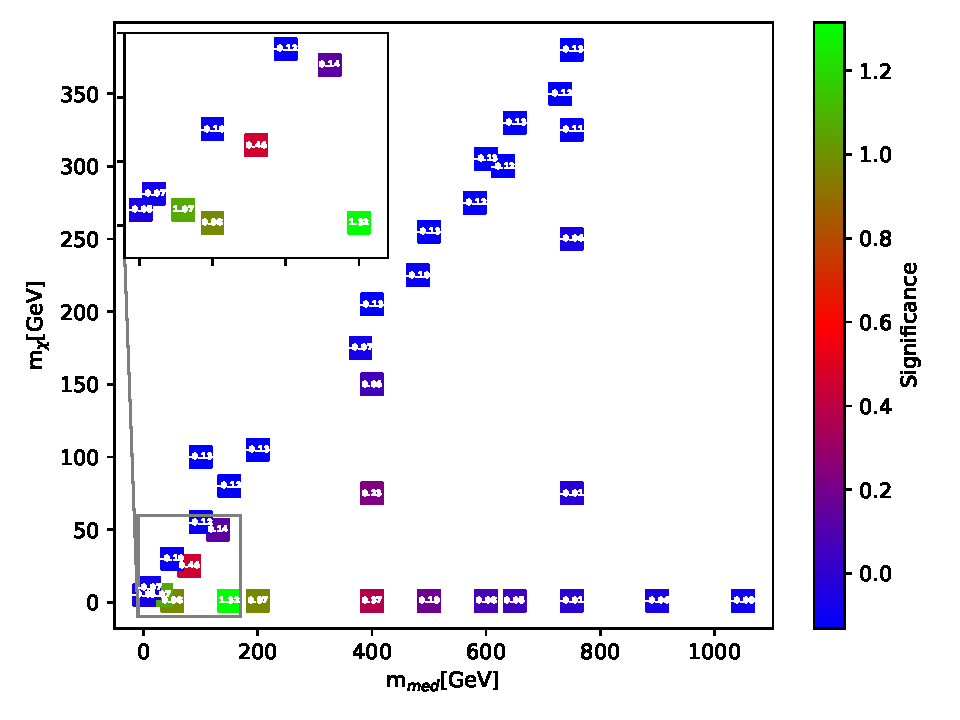
\includegraphics[width = \textwidth]{Figures/Significances/significance_NN_monoZ_All_level.pdf}
    \caption{Neural Network.}
        \label{fig:signAllmonoZNN}
    \end{subfigure}
    \caption{Significance plots for the mono-Z process where all features are used during training the ML models.}
    \label{fig:signAllmonoZ}
\end{figure}

The figure shows that the cut and count method are somewhat sensitive to signals with low mass splittings ($\Delta m < 100$ GeV). However, the ML methods are still more sensitive to a wider range of signals with low mass splittings. 



\subsection{Summarizing the results}
Overall the ML methods have better sensitivity compared to the cut and count method, especially for low mass splittings. This is also the case for the ML methods trained on low level and high level features, but they are not as good as the ones trained on all features. These results can be found in appendix \ref{sec:appsignificance}. 




\begin{comment}

- Dir slep: I LL  har ML litt dårlig sensitivitet en AL, HL har enda dårligere - forventet pga dir slep. Høy level variabler med her er ikke relevante for prosess. 

-Slep/snu: I LL  har ML hakket dårlig sensitivitet en AL, HL er ok, ikke så stor forskjell på LL og HL. 

- WW: LL < HL < AL. Interessant. 

- Mono-Z: Ganske bra LL og HL, nesten like bra som AL.



\end{comment}





